\documentclass[12pt]{article}

\usepackage{newunicodechar}
\usepackage{cite}
\usepackage{braket}
\usepackage{graphicx}
\usepackage{amsmath}
\usepackage{booktabs}
\usepackage{float}
\usepackage{subcaption}

\restylefloat{table}
\graphicspath{{./figures/}}

\newcommand{\hp}{H$_2^+$ }
\newcommand{\gr}{$\ket{g}$}
\newcommand{\us}{$\ket{u}$}
\newcommand{\psiv}{\begin{pmatrix}\Psi_1\\ \Psi_2\\ \end{pmatrix}}
\newcommand{\dt}{\Delta t}

\title{Dissociation dynamics of H$_2^+$ in XUV and IR laser fields}
\author{Tobias Becher, Lukas Blecher}
\date{March 2019}

\begin{document}
\bibliographystyle{unsrt}

\maketitle
\begin{abstract}
In this report we discuss the dissociative dynamics of the \hp ion under influence of an external IR-laser pulse. First on the vibrational eigenstates in the \hp electronic ground state are calculated. Following this the time evolution with and without the IR-pulse are simulated and a dissociation momentum analysis is done. 
\end{abstract}


\section{Introduction}
The starting point of the system discussed in the following is a \hp  ion in its electronic ground state. It is produced by an XUV laser pulse, that ionizes a H$_2$ molecule in its electronic and vibrational ground state. The so produced ion is in its electronic ground state \gr. However the vibrational wave packet is, according to the Franck-Cordon principle, represented by a superposition of excited \gr \ vibrational states. The initial wave packet of the \hp is the H$_2$ function. It moves on the \gr \ state until a second IR-pulse, with delay time $\tau$, leads to coupling with the \us \ state and the dissociation of the ion \cite{PhysRevA.93.012507,c107696046f943e78de27c893d23ac2f}.
\section{H$_2^+$ vibrational eigenstates}
As a first part of the analysis the vibrational eigenstates of \hp\ in the 
\gr\ state were calculated. To do so the Hamiltonian was represented on a grid and by using direct diagonalization solved.
The general form of the Hamiltonian is given by 
\begin{equation}\label{eqn:generalHamiltonian}
    \hat{H}=\frac{\hat{p}^2}{2\mu}+\hat{V}_{\ket{g}}
\end{equation}
$\mu$ being the reduced mass of the molecule and $V_{\ket{g}}$ the Born-Oppenheimer surface of the \hp\ electronic ground state.
The (time-independent) Schr\"odinger-equation (SDE) is now solved using a discrete matrix representation in which the Hamiltonian takes the form of

\begin{equation}\label{eqn:discresteHamiltonian}
    \hat H=\left({\begin{array}{cccccc}
   V(x_1)+\frac{1}{\Delta x^2} & \frac{-1}{2\Delta x^2} &0& \cdots & &\\
   \frac{-1}{2\Delta x^2} & V(x_2)+\frac{1}{\Delta x^2} & \ddots & & & \\
   0 &\ddots  &\ddots &&&\\
   \vdots&&&&&\\
  \end{array} } \right)
\end{equation}
\begin{figure}[htb]
    \centering
    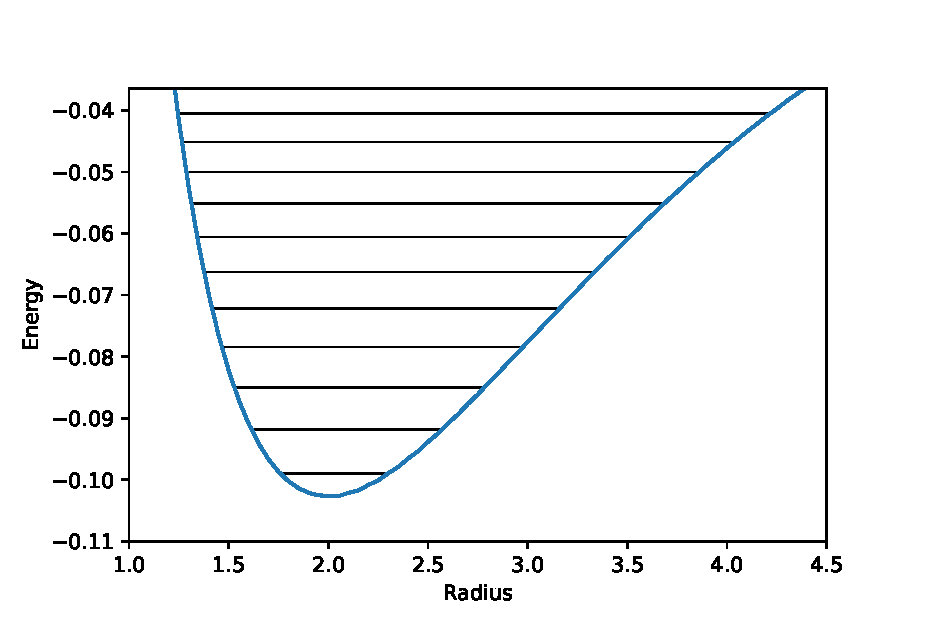
\includegraphics[width=1\textwidth]{vibEigenstates.eps}
    \caption{Vibrational eigenstates of $V_{\ket{g}}$ }\label{fig:vibStates}
\end{figure}
As seen in Figure \ref{fig:vibStates} the eigenvalues appear with a same spacing as the ones of the unperturbed quantum oscillator for lower levels. However for higher orders, the spacing shrinks, as the potential deviates more from an oscillator curve. The lowest vibrational eigenenergies are:
\begin{table}[H]\centering\label{tab:vibEnergies}
\begin{tabular}{@{}ccc@{}}
\toprule
n & a.u. & eV \\ \midrule
0&-0.0990&-2.693\\
1&-0.0918&-2.498\\
2&-0.0850&-2.312\\
3&-0.0784&-2.134\\\bottomrule
\end{tabular}
\caption{Eigenenergies in atomic units and eV}
\end{table}

\section{Time evolution without the laser coupling}
To simulate the vibrational dynamics of H$_2^+$, the initial H$_2$ wave function is used and propagated on the \gr\ surface. This corresponds to the dynamics of the system before the arrival of the IR-laser pulse. A split-step algorithm for the propagation was used, as introduced in the lecture. The Hamiltonian describing the system, is equal to \eqref{eqn:generalHamiltonian}.
The animation can be found under the name "propagation\_without\_IR-Laser.mp4"
in the folder.
Looking at the propagation, one oscillation period of the wave packet is visible. However, afterwards the wave packet appears to oscillate no further with only peaks rising and falling visible. A clear revival of the initial state is not visible (compare Fig.\ref{fig:withoutIR}).
\begin{figure}[H]
    \centering
    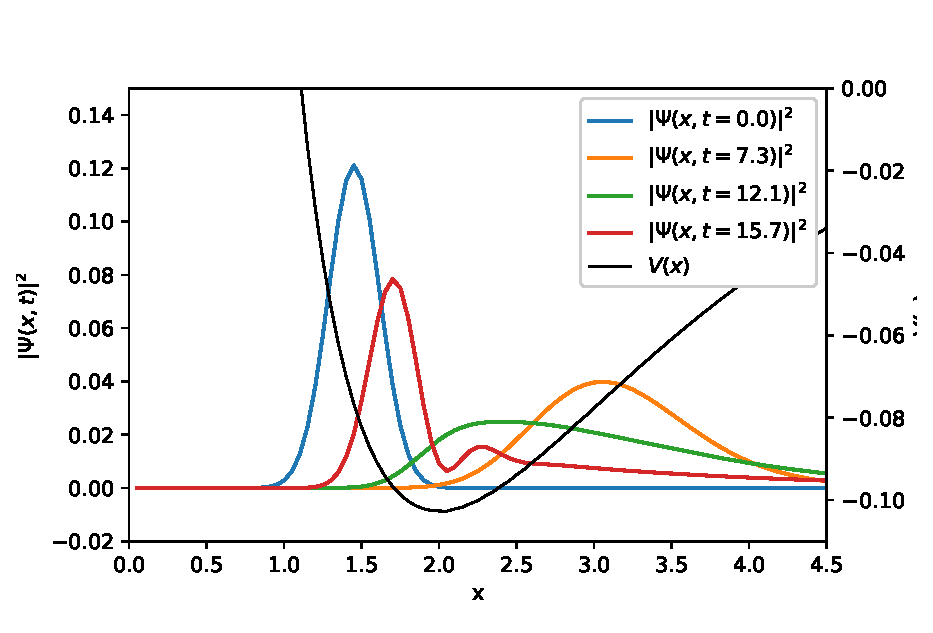
\includegraphics[width=1\textwidth]{woIR.eps}[]
    \caption{Time evolution of the ground state in $V_{\ket{g}}$ in atomic units}\label{fig:withoutIR}
\end{figure}


\section{Dissociative dynamics}
Following the initial dynamics a IR-pulse interacts with the system. The pulse couples  the known \gr \ state with the \us \ state. The latest is an electronic excited state. Considering the influence of the laser pulse, the time dependent Schr\"odinger equation of the system is given in \cite{PhysRevA.93.012507}
\begin{equation}\label{eqn:dissociativeDyn}
i
\frac{d}{dt}
\psiv
=
\begin{pmatrix}
\frac{\hat{p^2}}{2\mu}+V_g & -D\cdot E(t)\\
-D\cdot E(t) & \frac{\hat{p^2}}{2\mu}+V_u\\
\end{pmatrix}
\cdot
\psiv
\end{equation}
$V_g$ and $V_u$ are the Born-Oppenheimer surfaces of the two relevant states, D the element of the dipole matrix coupling the two states and E the laser-pulse.
Latest has the form of a cosine with a Gaussian envelope

\begin{equation}
   E(t)=E_\parallel \cdot \cos(\omega t) \cdot \exp \Bigl( -\frac{\left(t-\tau\right)^2}{2\sigma^2} \Bigr)
\end{equation}
The time evolution of this system is solved using a split-step algorithm. In contrast to the algorithm before there are now  two coupled equations that, in addition, are also time dependent. For this system the time step is given by \cite{doi:10.1063/1.465362}
\begin{equation}
\psiv (t+\Delta t)= \exp(-i[\Delta t\ \hat{T} + \Delta t\ \hat{V}(t+\Delta t /2)]) \cdot \psiv(t)
\end{equation}
Here  $\hat{T}$   is the kinetic Operator given by
\begin{equation}\hat T=
\begin{pmatrix}
\frac{\hat{p^2}}{2\mu}& 0\\
0 & \frac{\hat{p^2}}{2\mu}\\
\end{pmatrix}
\end{equation}
and $\hat{V}$ the time dependent potential operator
\begin{equation}
\hat V=
\begin{pmatrix}
V_g & -D\cdot E(t)\\
-D\cdot E(t) & V_u\\
\end{pmatrix}
\end{equation}
For the split step algorithm, the kinetic part remains unchanged- it is executed for $\Psi_1$ and $\Psi_2$ as if they were time independent not coupled equations.
However the potential step has to be adjusted. First on the potential is separated in a time dependent and an independent part.

\begin{equation}
\hat V=\underbrace{
\begin{pmatrix}
V_g & 0\\
0 & V_u\\
\end{pmatrix}}_{\hat V_c}
+ \underbrace{
\begin{pmatrix}
0 & -D\cdot E(t)\\
-D\cdot E(t) & 0\\
\end{pmatrix}}_{\hat V_t}
\end{equation}
The exponential of the potential step can be approximately expressed by
\begin{equation}
\exp(-i\dt\hat V)\approx \exp(-i\dt\hat V_c/2)\cdot \exp(-i \dt\hat V_t) \cdot \exp(-i \dt\hat V_c/2)
\end{equation}
The exponents with the time independent potential do not represent a problem, as they are diagonal. On the other hand the time dependent one needs to be expressed otherwise before, as it is not diagonal.
As a solution to this problem the $\hat V_t$ matrix is represented by 
\begin{equation}
\hat V_t=\hat U^*\hat D\hat U
\end{equation}
with D being a diagonal and U a unitary matrix.
To find the according matrices the eigenvalues and eigenvectors of $\hat V_t$ are calculated, which are 
\begin{subequations}
\begin{align}
D\cdot E(t) &&\text{and} && \begin{pmatrix}
a\\
a\\
\end{pmatrix}
\end{align}
\begin{align}
-D\cdot E(t) && and & &\begin{pmatrix}
b\\
-b\\
\end{pmatrix}
\end{align}
\end{subequations}
a and b being arbitrary values.
With these the U and D matrix have the form of
\begin{subequations}
\begin{equation}
\hat U= \frac{1}{\sqrt{2}}\begin{pmatrix}
1 & 1\\
1 & -1\\
\end{pmatrix}
\end{equation}
\begin{equation}
\hat D=\begin{pmatrix}
D \cdot E & 0\\
0 & -D \cdot E\\
\end{pmatrix}
\end{equation}
\end{subequations}
Using all the above expressions the potential step of the split step algorithm takes the form of
\begin{equation}
\exp(-i\dt\hat V)\approx \exp(-i\dt\hat V_c/2)\cdot\hat U^*\cdot \exp(-i \dt\hat D)\cdot\hat U\cdot \exp(-i \dt\hat V_c/2)
\end{equation}
with which the time evolution can be solved numerically. The result of the time evolution can be found in "propagation\_with\_IR-Laser.mp4".
The same dynamic as before is visible, however with a small wave packet appearing on the \us\ state. This leads to the conclusion that the coupling by the laser has a small influence on the system in the simulation. However, comparing with the results of \cite{PhysRevA.93.012507}, a clear separation of the ion would be expected. A possibility for the differences could be a divergence of the simulation to reality. 
\begin{figure}
	\centering
	\begin{subfigure}{0.4\textwidth} % width of left subfigure
		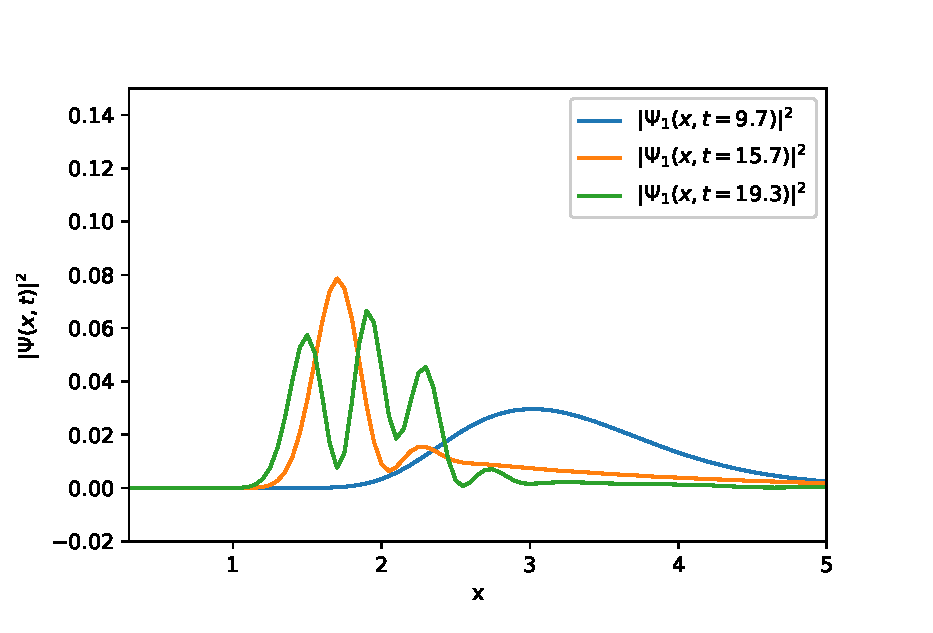
\includegraphics[width=\textwidth]{withIR_1.eps}
		\caption{$|\Psi_1(x,t)|^2$} % subcaption
	\end{subfigure}
	\vspace{1em} % here you can insert horizontal or vertical space
	\begin{subfigure}{0.4\textwidth} % width of right subfigure
		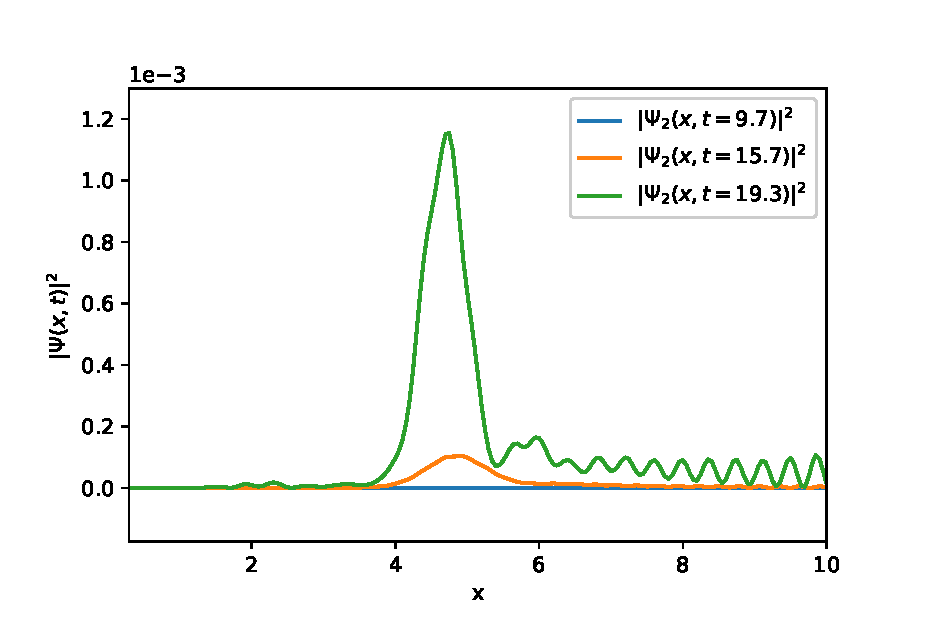
\includegraphics[width=\textwidth]{withIR_2.eps}
		\caption{$|\Psi_2(x,t)|^2$} % subcaption
	\end{subfigure}
	\caption{Time evolution according to \eqref{eqn:dissociativeDyn} for $\Psi_1$ and $\Psi_2$ in atomic units} 
\end{figure}

\bibliographystyle{plain}
\bibliography{references}
\end{document}
